\chapter{Under-surface prediction}
%The following experiment now considers a surface to predict the dynamic at hidden layer under the surface.
%The goal of the experiment is to have an idea about the limitations on this specific task. The following aspects are relevant in the research:
%\begin{itemize}
%    \item How does the length of the input affect the quality of the results in dependency of the depth.
%    \item Is it an advantage to consider the dynamic at the surface in the future to predict a hidden layer.
%    \item How much does random behaviour affect the quality of the prediction.
%    \item Does spatial correlation between two layer, correlate with the quality of the prediction.
%\end{itemize}

%Each of these questions aim to build a guideline for future work on a heart simulation, which obviously has a much more complicate structure. This experiment under thinkable simple conditions has the function as a playground to test which parameter are critical, and which configuration has the best compromise.

% What, in broad terms
This chapter is about the second numerical experiment. The basis for it is a 3D-simulation of the time evolution of an excitable medium. The question is to what extent a machine learning model respectively a neural network can predict a system quantity inside of the 3D structure which is not \textit{visible} from outside. The input to the neural network and its prediction are values of the same system quantity, where the input is recorded on the surface of the 3D structure over a period of time. Here, \textit{not visible} means that the neural network has no explicit information about the data inside the 3D structure that it is supposed to predict. Only on the basis of the surface it is to extrapolate these. The posing of this problem is motivated by a possible transfer to heart dynamics. It would be a matter of inferring the inner dynamics from the surface dynamics which results from the electrical activity of the heart muscle cells. 

In general, one wants to get as much information from the heart's activity as possible with minimally invasive or non-invasive measurement methods to make an intervention to obtain this information as low-risk and cost-effective as possible. While the first experiment was about drawing conclusions about the electrical activity at the surface of the heart from the ECG signals, one prospect of this experiment is to predict the interior electrical activity, based on the heart's surface.

% Storyline
%While the previous experiment was about information gain of the surface of the heart, based on an ECG-signal, this experiment now takes into account the surface to get information about the system under the surface.

% Previous work
Some experiments have been done by [xx] or [yy]. While these approaches are based on real data and , in this work I will go a step back and want to study the limits of machine learning models that faces up to the task mentioned above, while having \textit{perfect} surface information. \textit{Perfect} means here, unlike in real experiments, that the data does not have any noise\footnote{If we ignore the numerical error.}. Furthermore, with choosing a cube as comparatively simple geometry, I regard this as a base study about the limitations of machine learning models in this kind of problem. This numerical experiments tests two different sequence-to-sequence LSTM architectures on two different parameter sets within the model for excitable media where one builds \textit{concentric waves} and the other \textit{breaking spiral waves}, as visualized in figure [xx]. Details concerning the characteristics of these regimes are explained in section [yy]

How a possible transfer of this experiment to biological data can be realized and to what extent it would build on the results of this study is discussed in chapter xx.

% Exact input and output

% Excitable media model and hyperparamter
% Barkley, and two regimes, 

% Machine learning models
% LSTM and STLSTM

% Leserorientierung

% Simulation, (chaos, concentrisch)
% Training of neural network in general,
% Optimal parameter search (also with respect to graphics card, see appendix)
% Study: Varying time-span from input. The more time steps the better? (-->till certain point not better)
% Comparison between LSTM and STLSTM

% Zu erklären: Two regimes, 

\section{Methods}\label{cap:diver_methods}
Goal is to train a machine-learning model which takes into account the time evolution of the $u$-value of the Barkley model \cite{Barkley_2008} at the surface, to predict at a certain time point the $u$-value under the surface. In this chapter I introduce the process of generating training- and validation data and elaborate some characteristics of the simulations.

\subsection{Model}
There are various models to describe the heart dynamic but since this experiments goal is to reconstruct hidden regions under the surface qualitatively, the model does not have to describe the heart dynamic as accurate as possible. In this work the Barkley model is used, which is a system of two coupled differential equations which build a reaction-diffusion system. It is a comparably\footnote{Compared for example with the Hodgkin-Huxley model which consists of three coupled differential equations.} simple model and consists of two variables $u$ and $v$ which are dependent on the equations

\begin{align}
    \frac{\partial u}{\partial t}&=D\cdot \nabla^2u+\frac{1}{\varepsilon}(1-u)\left(u-\frac{v+b}{a}\right)\notag\\
    \frac{\partial v}{\partial t}&=u^{\alpha}-v.\notag\\
\end{align}

The parameter $\epsilon$ controls . A bigger value for $a$ increased the excitation duration while an increasing fraction between $b$ and $a$, $\frac{b}{a}$, results to a larger excitability threshold. In this work the value for $\alpha$ is set to 1. The exact values for both regimes are in table (\ref{tab:simulation_parameter}).

\subsubsection{Simulation}
The Barkley-model will be simulated in three dimensions in which the discretised diffusion operator $\nabla^2$ is here described through a 7-point stencil such that

\begin{align}
    \left(\nabla_7^2u\right)_{i,j,k}=\frac{u_{i-1,j,k}+u_{i+1,j,k}+u_{i,j-1,k}+u_{i,j+1,k}+u_{i,j,k-1}+u_{i,j,k+1}-6u_{i,j,k}}{\Delta s^2},
\end{align}

where the indices $i$,$j$ and $k$ stand for the discretised position within the $x$-$y$-$z$-cube and $\Delta s$ the spatial discretisation. A simulation step in time will be calculated through the explicit Euler method with

\begin{align}
    u(t+1)&=u(t)+\Delta t\frac{\partial u(t)}{\partial t}\notag\\
    v(t+1)&=v(t)+\Delta t\frac{\partial v(t)}{\partial t}.\notag\\
\end{align}

that a time-step within the Barkley model is described as 

\begin{align}
    u(t+1)_{i,j,k}&=u(t)_{i,j,k}+\Delta t\cdot\left(D\cdot \left(\nabla_7^2u\right)_{i,j,k}+\frac{1}{\varepsilon}(1-u(t)_{i,j,k})\left(u(t)_{i,j,k}-\frac{v(t)_{i,j,k}+b}{a}\right)\right)\notag\\
    v(t+1)_{i,j,k}&=v(t)_{i,j,k}+\Delta t\cdot\left(u(t)_{i,j,k}^{3}-v(t)_{i,j,k}\right)\notag\\
\end{align}

The hyperparameter $a$, $b$, $\varepsilon$, $\Delta t$ and $\Delta s$ are arbitrary chosen for two regimes, in which one builds concentric waves and the other shows a chaotic behaviour. The exact values are shown in table (\ref{tab:simulation_parameter}). The simulation is implemented in python with orientating on the code for a 2D Barkley simulation by Roland Zimmermann \cite{zimmermann}.
%\subsection{Data-assimilation}
\subsubsection{Hyperparameter and simulation size}

\begin{table}[h]
    \centering
    \begin{tabular}{|c|c|c|}
    \hline
    & Non-chaotic & chaotic\\
    \hline
    $a$ & 0.6 & 1.0 \\
    \hline
    $b$ & 0.01 & 0.15 \\
    \hline
    $\epsilon$ & 0.02 & 0.02 \\
    \hline
    $\Delta t$ & 0.01 & 0.01 \\
    \hline
    $\Delta s$ & 0.1 & 0.1 \\
    \hline
    $\alpha$ & 1 & 1\\
    \hline
    \end{tabular}
    \caption{Barkley simulation configurations.}
    \label{tab:simulation_parameter}
\end{table}

The parameter set for 'non-chaotic' is adjusted to build concentric waves (as visualized in figure xx), while the chaotic regime produces breaking spiral waves. The parameter adjustment for $a$ and $b$ is based on a paper by Alonso et al. \cite{alonso_taming_2003} in which they study the parameter-space of the Barkley model and their influence within a 3D-simulation.

These two parameter regimes 
The parameter are specifically chosen to generate
Both simulations are embedded on the cube with 120 unit in each dimension. 

\subsubsection{Characteristic units}

To have a more intuitive understanding about time- and spatial sized which are taken into account by the models I apply characteristic dimensions as following:

\begin{itemize}
    \item Length $L_c$: The characteristic length $L_c$ is defined by average thickness along the normal of a wave front. Here it is estimated manually by taking the average from 32 measurements $\iota=\overline{(\iota_1,...,\iota_{32})}$. The length follows to $L_c=\iota\cdot\Delta\text{s}$.
    \item Velocity $V_c$: The velocity is measured by counting the amount of discrete length units $\Delta s$ which are passed per discrete time step $\Delta t$. To minimize the error, the distance is measured after 64 time-steps, and the average of 32 of these measurements build the characteristic velocity as $V_c=\nu\cdot\Delta\text{s}/\Delta\text{t}$.
    
    \item Time $T_c$: The characteristic time is applied by the time a wave needs to travel the characteristic length. It follows the time according to $T_c=L_c/V_c\equiv\iota/\nu\cdot\Delta\text{t}=:\tau\cdot\Delta\text{t}$.
    %Why the connection of the length and time is motivated by the problem definition is explained in chapter (231).
\end{itemize}

The resulting values for $\iota$, $\nu$ and $\tau$ are shown in table (\ref{tab:characteristic}). 

\begin{table}[h]
    \centering
    \begin{tabular}{|c|c|c|}
    \hline
    & 1: Non-chaotic & 2: chaotic\\
    \hline
    $\iota$ & 10.50$\pm$1.45 & 3.15 \\
    \hline
    $\nu$ & 0.155$\pm$0.041 & 3.15 \\
    \hline
    $\tau$ & 67.74$\pm$20.24 & 3.15 \\ % 67.74
    \hline
    $L_c$ & 1.05$\pm$0.15 & 3.15 \\ % 67.74
    \hline
    $V_c$ & 1.55$\pm$0.41 & 3.15 \\ % 67.74
    \hline
    $T_c$ & 0.68$\pm$0.20 & 3.15 \\ % 67.74
    \hline
    \end{tabular}
    \caption{Characteristic dimensionless units for the two Barkley configurations.}
    \label{tab:characteristic}
\end{table}

Intuitively, a wave-front which propagates along the normal of the surface in a depth of $\iota\cdot\text{ds}$, needs in average $\tau$ discrete time steps to be recognisable at the surface. %The time a structure needs to be visible in future time step at surface is a considered quantity in the experiment. %In chapter (RESULTS) I will show that if the model takes into account future time steps, it is able to reconstruct non-surface structures at a given time point in the past.

\subsection{Generating data and preprocessing}
% Simulation output --> what to do for model
% float64 to int8
% - reshape to single datapoints, save as pytorch-dataset
%120x120x120 --> (X,y) == (B,T,D,H,W), 
%\section{Seq2Seq neural network for under-surface prediction}

The following described procedure of data generation and preprocessing is the same for both regimes. The only difference is the adjusting of hyperparameters according to table (\ref{tab:simulation_parameter}).

\subsubsection{Data generation}
As mentioned before, I consider in the experiment the $u$ value of the Barkley model. Since the cube has an expansion of 120 discretised units in each spatial dimension, a snapshot of the $u$ value is a tensor of order 3 with a dimensionality of (120,120,120)=(depth, height, width). 
In a single simulation each snapshot is recorded after 16 discrete time-steps from the previous snapshot over a span of 512 steps. Therefore, each simulation saves a tensor with the dimensionality of (32,120,120,120). The recording starts after an initial phase of 2048 time steps. Basis for the preprocessing step, which I explain in the following, are 256 of these simulations for each regime (concentric and chaotic). Here I use $X$ to describe the data the machine learning model gets as input to predict $y$.


\subsubsection{Preprocessing}
% X and y describing
Since a cube has 6 sides, here each simulation produces 6 time-series from the surface. The corresponding $y$-data is a tensor which saves the $u$-value for the next lower layers below the respective surface. The maximal depth is set at 32 discrete spatial units. Therefore, from 256 single simulations, one gets $256\cdot6=1536$ X-y-pairs with $X\in R^{32\times1\times120\times120}$ and $y\in R^{1\times32\times120\times120}$. It is divided into a training-set (1024 pairs) and validation set (512 pairs). Note that the dimensions stand for (time-steps$\times$depth$\times$height$\times$width). The $X$-data includes only the surface of the cube, therefore the depth is always 1, while $y$ is the prediction at a certain time-step till a maximal depth of 32.
The data within the simulations are computed as float64 (means each single value needs 64 bit of storage with the float data type). Nonetheless it is possible without a great loss on information to convert the data into one-byte-integers (int8) to save storage. Therefore, $X$ and $y$ are rescaled into the range of int8 (-127 to 128). 

Within the training process, the data again has to be rescaled into the range from 0 to 1. This is done with the help of a pytorch dataloader, whose functionality is explained in \ref{cap:pytorch}.

\subsection{C-LSTM and ST-LSTM}
In section (\ref{cap:seq2seq}) a general design of sequence-to-sequence models with recurrent neural networks was introduced. In this section, I present the exact composition of the models used in this experiment. The two models differ only in the implementation of their recurrent cells, which are the C-LSTM cell (see section \ref{cap:CLSTM}) and the ST-LSTM cell (see section \ref{cap:STLSTM}).

The models are based on the same architecture as visualized in figure (\ref{fig:seq2seq}). The encoder- (embedding) and decoder-networks (colored green in figure (\ref{fig:seq2seq})) are time distributed, which means that the same network is used separately for each time point of an input sequence. Encoder and decoder are convolutional neural networks whose architecture is visualized in figure (\ref{fig:encoder}) and (\ref{fig:decoder}). Some convolutional layers have a stride-parameter of 2, which reduces the spatial dimensionality by the factor of two. Therefore, with an input $X$ with $X\in R^{\text{batch}\times\text{time-steps}\times\text{depth}\times\text{height}\times\text{width}}$, the encoder reduces it to $X_{\text{out}}\in R^{\text{batch}\times\text{time-steps}\times\text{features}\times\text{height/2}\times\text{width/2}}$. Note, that instead of \textit{depth}, the third dimension represents now the number of channels, which is a hyperparameter of a convolutional layer as introduced in section (\ref{cap:multichannel}). The value is always set for all convolutional layers within the encoder and decoder to 64.

\begin{figure}[!tbp]
  \centering
  \begin{minipage}[b]{0.4\textwidth}
    \includegraphics[width=\textwidth]{figures/encoder.png}
    \caption{Encoder}
    \label{fig:encoder}
  \end{minipage}
  \hfill
  \begin{minipage}[b]{0.4\textwidth}
    \includegraphics[width=\textwidth]{figures/decoder.png}
    \caption{Decoder}
    \label{fig:decoder}
  \end{minipage}
\end{figure}

\subsection{Optimal hyperparameter search}
While the architecture of the two approaches (C-LSTM and ST-LSTM) will be considered as given, I search for the optimal hyperparameter for the training process. These are the loss-function, learning rate, batch size and the optimizer. Table (\ref{tab:gridsearch}) shows the values of the hyperparameters that are varied, as well as the ideal parameter combination.

\begin{figure}[ht]
    \center
    \includegraphics[width=0.99\textwidth]{figures/sweep_clstm.png}
	\caption{Results of a grid-search with 4 varying hyperparameter. The hyperparameter in this graphic are sorted by its influence to the loss from less important (left) to more important (right) (the importance is sorted by random forest feature importance to calculate how much a hyperparameter choice played a role in the result according to the metric). The parameter-variations and best combination are in table (\ref{tab:gridsearch}). The loss is calculated after one epoch with 1024 examples.}
	\label{fig:sweep_clstm}
\end{figure}

\begin{table}[h]
    \centering
    \begin{tabular}{|c|c|c|}
    \hline
    Parameter & Values & Best value\\
    \hline
    \hline
    Loss function & MSE, MAE & MSE\\
    \hline
    Learning rate & $\{1,2,3,5\}\cdot10^{-4}$, $\{1,2,3\}\cdot10^{-3}$ & $10^{-4}$\\
    \hline
    Batch-size & 2,4,6,8 & 4\\
    \hline
    Optimizer & SGD\footnote{Stochastic gradient descent}, Adam & Adam \\ % 67.74
    \hline
    \end{tabular}
    \caption{Characteristic dimensionless units for the two Barkley configurations.}
    \label{tab:gridsearch}
\end{table}

\section{Specific studies}
% Including varying time-steps, comparison.
% Qualitative results, can structures be detected?
% Performance on chaos regime, plus using ST-LSTM
In this work I consider four studies. Included are the two described models C-LSTM and ST-LSTM to perform tasks within two regimes. All studies have in common, that a machine learning model takes as input a temporal sequence of the $u$-value from the Barkley model, which is one side of the surface of the 3D simulation with the shape of a cube.

\subsection{Influence of the input-sequence length}
First, I vary the length of the temporal sequence as input. Goal of this study is to find in 

\subsection{Qualitative detection of hidden structures}
In the second study I figure out if hidden structures can be deteced by 
\subsection{Comparison C-LSTM, ST-LSTM}
\subsection{Performance of chaotic regime}

First, I vary the length of the time interval that the models use as a basis for their prediction. In excitable media, an excitation has an increasing global influence with time passed. This leads to the assumption that excitations below the surface have an influence on the surface dynamics after a certain time passed. The first study is about the question if or rather in which amount this influence can affect the prediction accuracy. The characteristic velocity, which I introduced in chapter 4, plays an important role in this process. Since in both regimes (see table xx) build wave-fronts, the average speed of these wave fronts is used as characteristic velocity. 

\section{Results and validation}
Influence of the input-sequence length

The results are separated into three parts. Firstly I show the general ability of detecting hidden structures with a surface-sequence. These results are based on experiments which are performed only with the C-LSTM in regime 1 (see table (\ref{tab:simulation_parameter}) at \textit{non-chaotic} for the exact Barkley-hyperparameter).

The in the second part, I compare the results of C-LSTMs and ST-LSTMs
% Plot example: Time-steps sättigung, depth of 5, + depth of 

The plot show curvature which are smoothed with the Savitzy-Golay filter \cite{Savitzky1964SmoothingAD} to increase the visibility of the curves. Without the filter they would be very noisy.

%\begin{figure}[ht]
%    \center
%    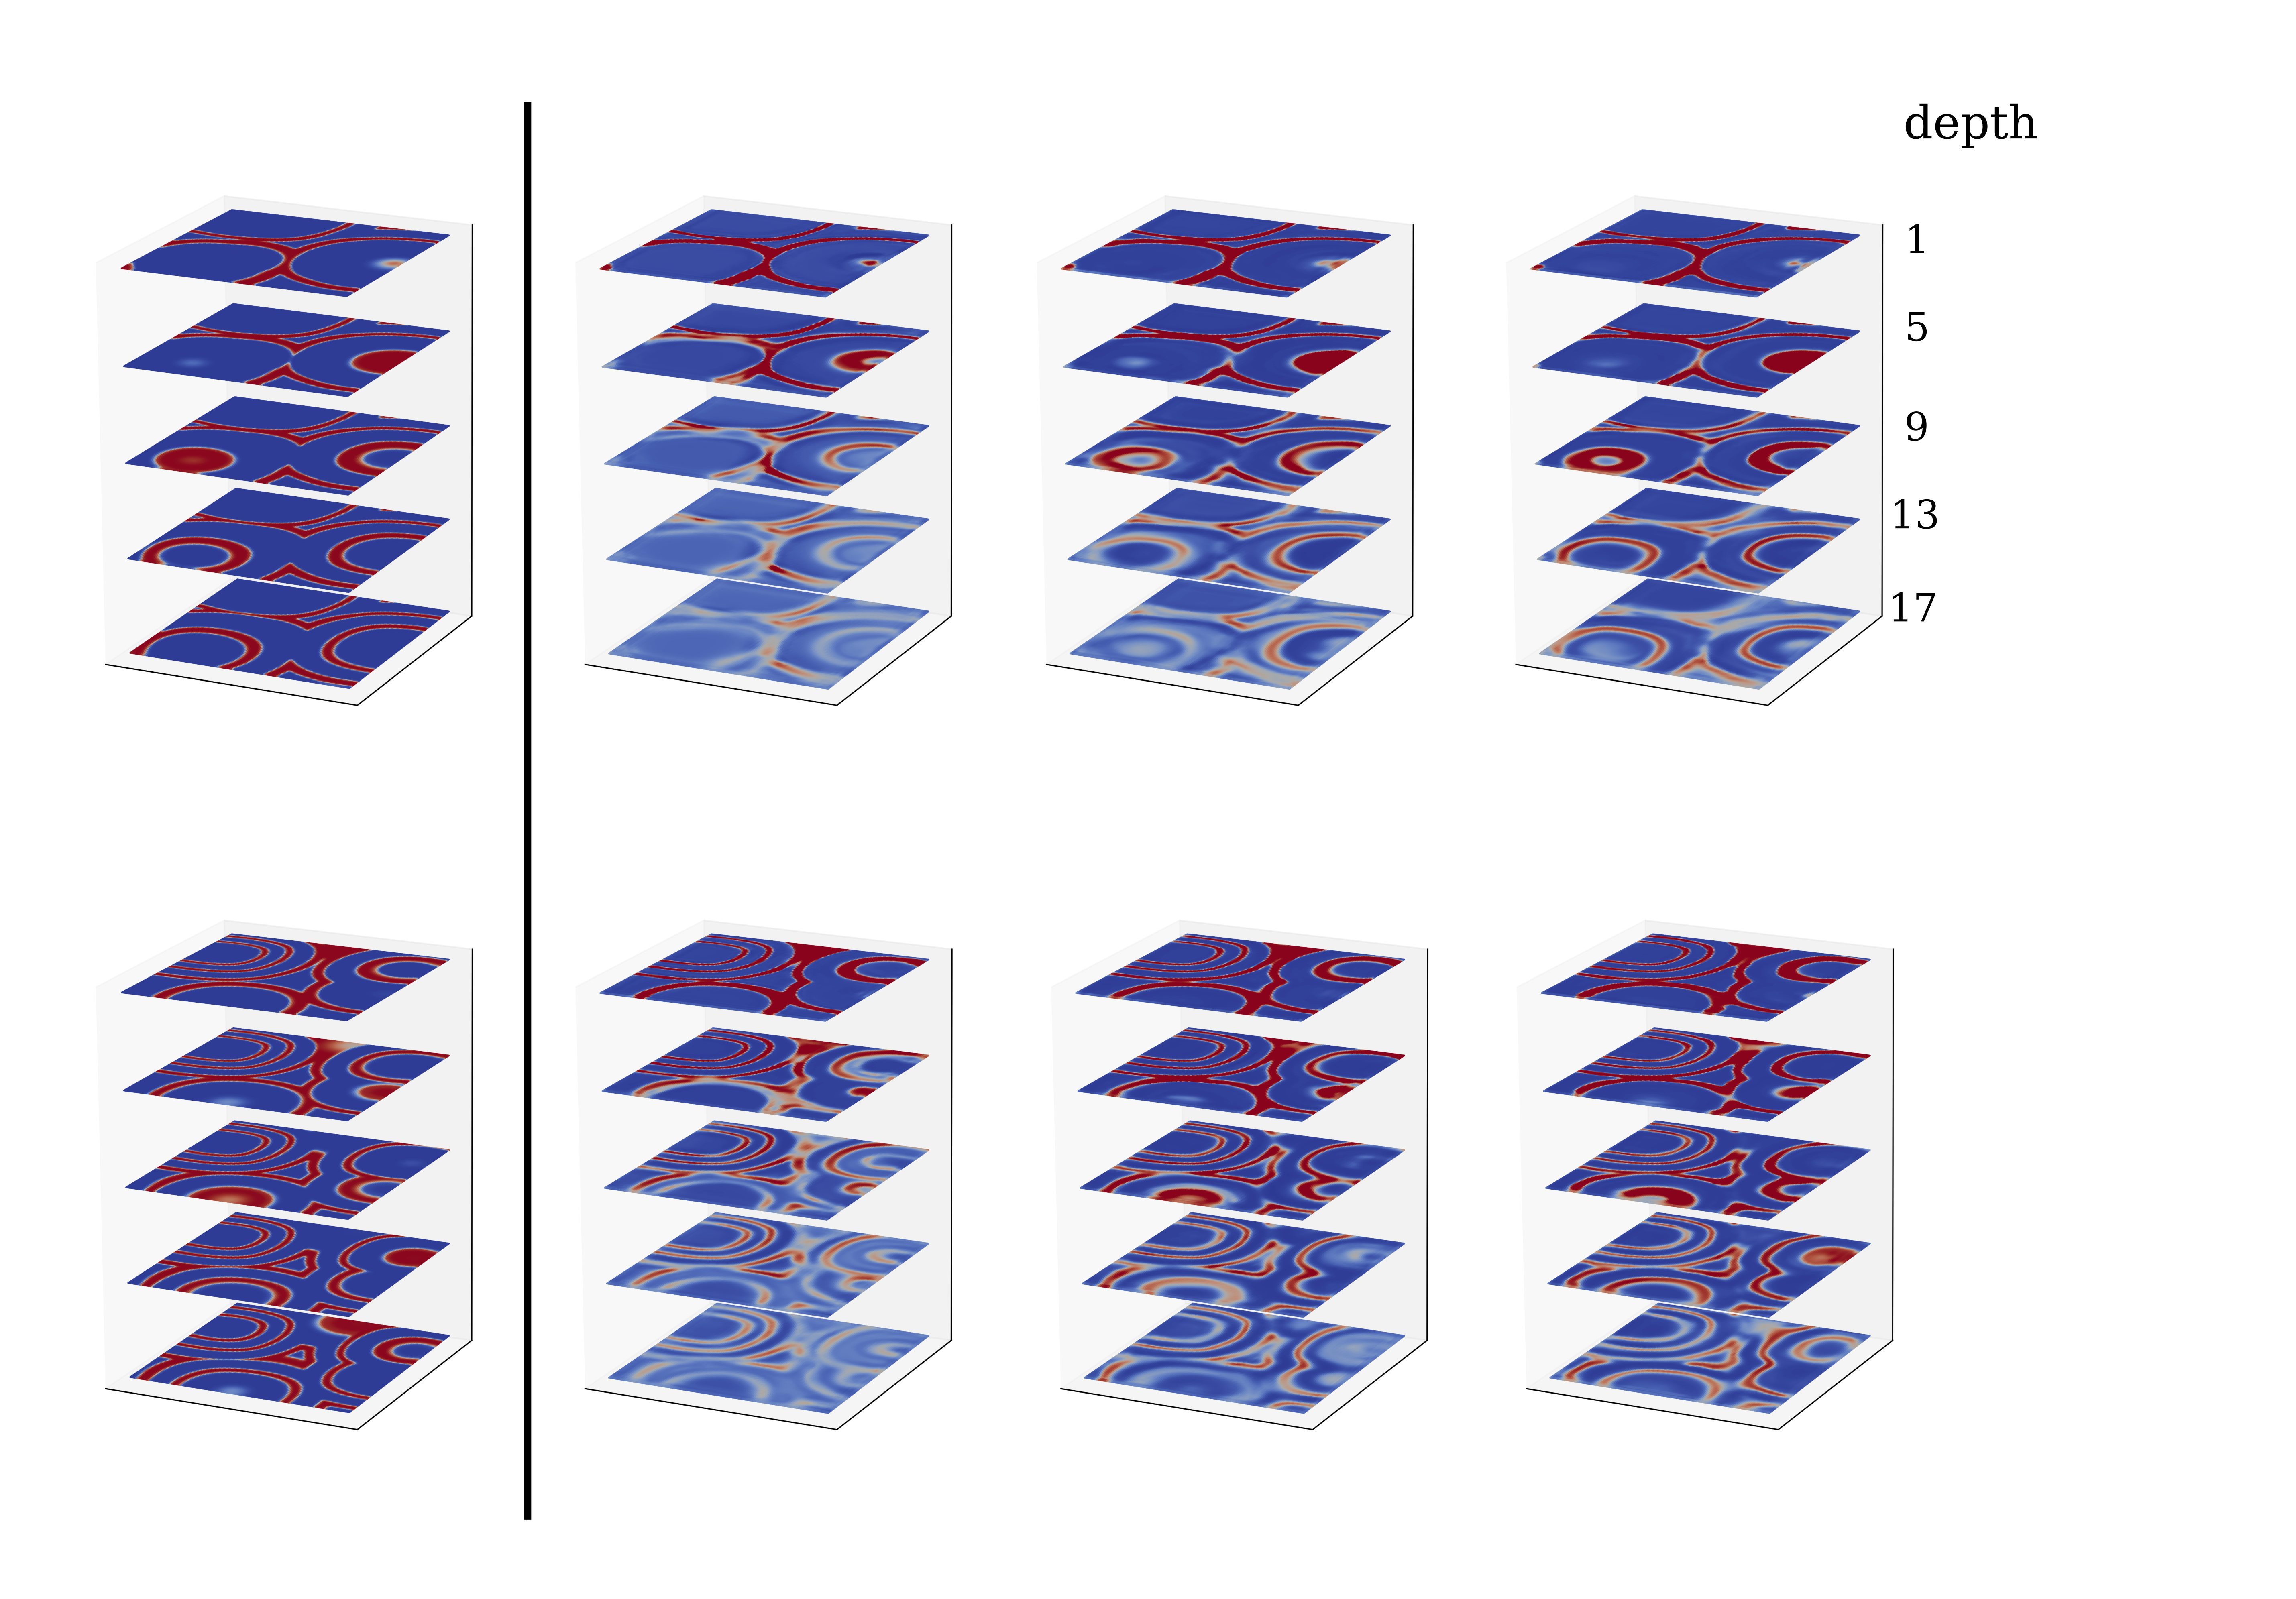
\includegraphics[width=0.99\textwidth]{figures/cubeplots1.png}
%	\caption{Hyperparameter search, sorted by importance. The validation loss is calculated after one epoch with 1024 examples. The model considers in the output a depth of 8 with having an input sequence of length 8.}
%	\label{fig:sweep_clstm}
%\end{figure}

\begin{figure}[!htb]
    \center
    \includegraphics[width=0.95\textwidth]{figures/CLSTM_p361_d32_t_1_8_32.png}
	\caption{Comparison, a point is visualized as long its value is over 0.5.Comparison, a point is visualized as long its value is over 0.5.Comparison, a point is visualized as long its value is over 0.5.}
	\label{fig:clstm_3d_p361}
\end{figure}

\begin{figure}[!htb]
    \center
    \includegraphics[width=0.95\textwidth]{figures/CLSTM_p26_d32_t_1_8_32.png}
	\caption{Comparison, a point is visualized as long its value is over 0.5.}
	\label{fig:clstm_3d_p26}
\end{figure}

%\section{Discussion}
%\subsection{iECG}
%\subsection{Under-surface predictor}
\textbf{What are the results}
What is the research usable for:
    - A study how good models work in this kind of problem, if it is even possible to detect hidden structures. And the work shows, it definitely is able to detect some of these structures under good circumstances and not in real time because it needs data from the future. Nonetheless some patterns can periodically. 

In a periodic dynamic, is it enough to have the surface-data? 
What is the core of the problem in terms of machine learning?
What is proven?
How can the results be useful for future work?
    - Can the models respectively the problem formulation be generalized, for example for a more complex geometry with the topological description of a doughnut.
How can approaches be embedded in the big field of machine learning 
    - shows one approach with is proven in a number of different fields to be able to build a state-of-the-art model or was state-of-the-art in a certain time.
    


